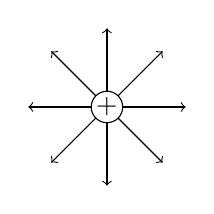
\begin{tikzpicture}
	%\draw[lightgray] (-2,-2) grid (2,2);
	\coordinate (A) at (0,0);
	%\draw (0,0) circle (1); 
	\draw[->] (A) -- (0.707,0.707);
	\draw [->] (A) -- (0,1);
	\draw[->] (A) -- (-0.707,0.707);
	\draw[->] (A) -- (-1,0);
	\draw[->] (A) -- (-0.707,-0.707);
	\draw[->] (A) -- (0,-1);
	\draw[->] (A) -- (0.707,-0.707);
	\draw[->] (A) -- (1,0);
	\fill[white] (A) circle (0.2cm);
	\draw (A) circle (0.2cm) node[]{$+$};
\end{tikzpicture}
